\chapter{Referencial teórico}\label{chapter:referencial_teorico}

% -----------------------------------------------------------------------------
% Capítulo 2.1 - IoT
% -----------------------------------------------------------------------------
\section{IoT}

Nos últimos anos, observou-se a ascensão de dispositivos inteligentes, dispositivos que se conectam à Internet. Esses dispositivos se comunicam entre si, possuem sensores e outras tecnologias. Em termos simples, define-se IoT como uma rede de itens - cada um com sensores integrados - que são conectados à Internet \cite{ref:003}.

Aprofundando, IoT também pode ser definido como uma rede que engloba um sistema de dispositivos de computação inter-relacionados, máquinas mecânicas e digitais, objetos, animais ou pessoa, e a capacidade de transferir dados através de uma rede sem a necessidade de interação entre humanos \cite{ref:004}. A presença de tecnologias de nuvem, \textit{big data} e redes móveis, por exemplo, em redes de IoT permite o compartilhamento e a coleta de dados com o mínimo de intervenção humana \cite{ref:005}. Pode-se listar as seguintes tecnologias como as protagonistas no crescimento do uso da tecnologia IoT:

\begin{itemize}
    \item Acesso a tecnologia de sensores de baixo custo e baixa potência;
    \item Conectividade;
    \item Plataformas de computação em nuvem;
    \item Aprendizado de máquina e análise avançada;
    \item Processamento de linguagem natural (Amazon Alexa, por exemplo).
\end{itemize}

Uma característica comum dos dispositivos IoT é a necessidade de componentes de interface para a interação com o mundo físico. Alguns exemplos de componentes de interface são:

\begin{itemize}
    \item Teclado, botões e microfones;
    \item Alarmes, visores e alto-falantes;
    \item Sensores;
    \item Atuadores;
\end{itemize}

% -----------------------------------------------------------------------------
% Capítulo 2.2 - Computação em nuvem com a AWS
% -----------------------------------------------------------------------------
\section{Computação em nuvem com a AWS}

A Amazon Web Services, Inc. (AWS) é uma empresa subsidiária da Amazon responsável por fornecer a seus clientes plataformas para a computação em nuvem sob demanda via Internet. Empresas fazem uso desse serviço para a criação e execução de aplicações virtuais sem um custo inicial, uma vez que a AWS tem o \textit{pay-as-you-go} como modelo de precificação. Ou seja, o cliente faz o pagamento conforme o uso \cite{ref:006}. Em 2022, a AWS é capaz de oferecer a seus clientes mais de duzentos serviços em nuvem nas áreas de tecnologias de computação, banco de dados, \textit{machine learning}, IoT, inteligência artificial etc \cite{ref:007}.

Ademais, a AWS conta com mais de 410 pontos de presença em mais de 90 cidades e 48 países \cite{ref:008}. Esse modelo de região e zona de disponibilidade da AWS foi reconhecido pelo Gartner, empresa de pesquisa e consultoria em TI, como o método recomendado para executar aplicativos corporativos que exigem alta disponibilidade \cite{ref:009}. A \autoref{fig:aws_zone} contém um mapa com as redes de presença da AWS, por região.

\begin{figure}[htbp]
    \centering
    \caption{Redes de presença da AWS.}
    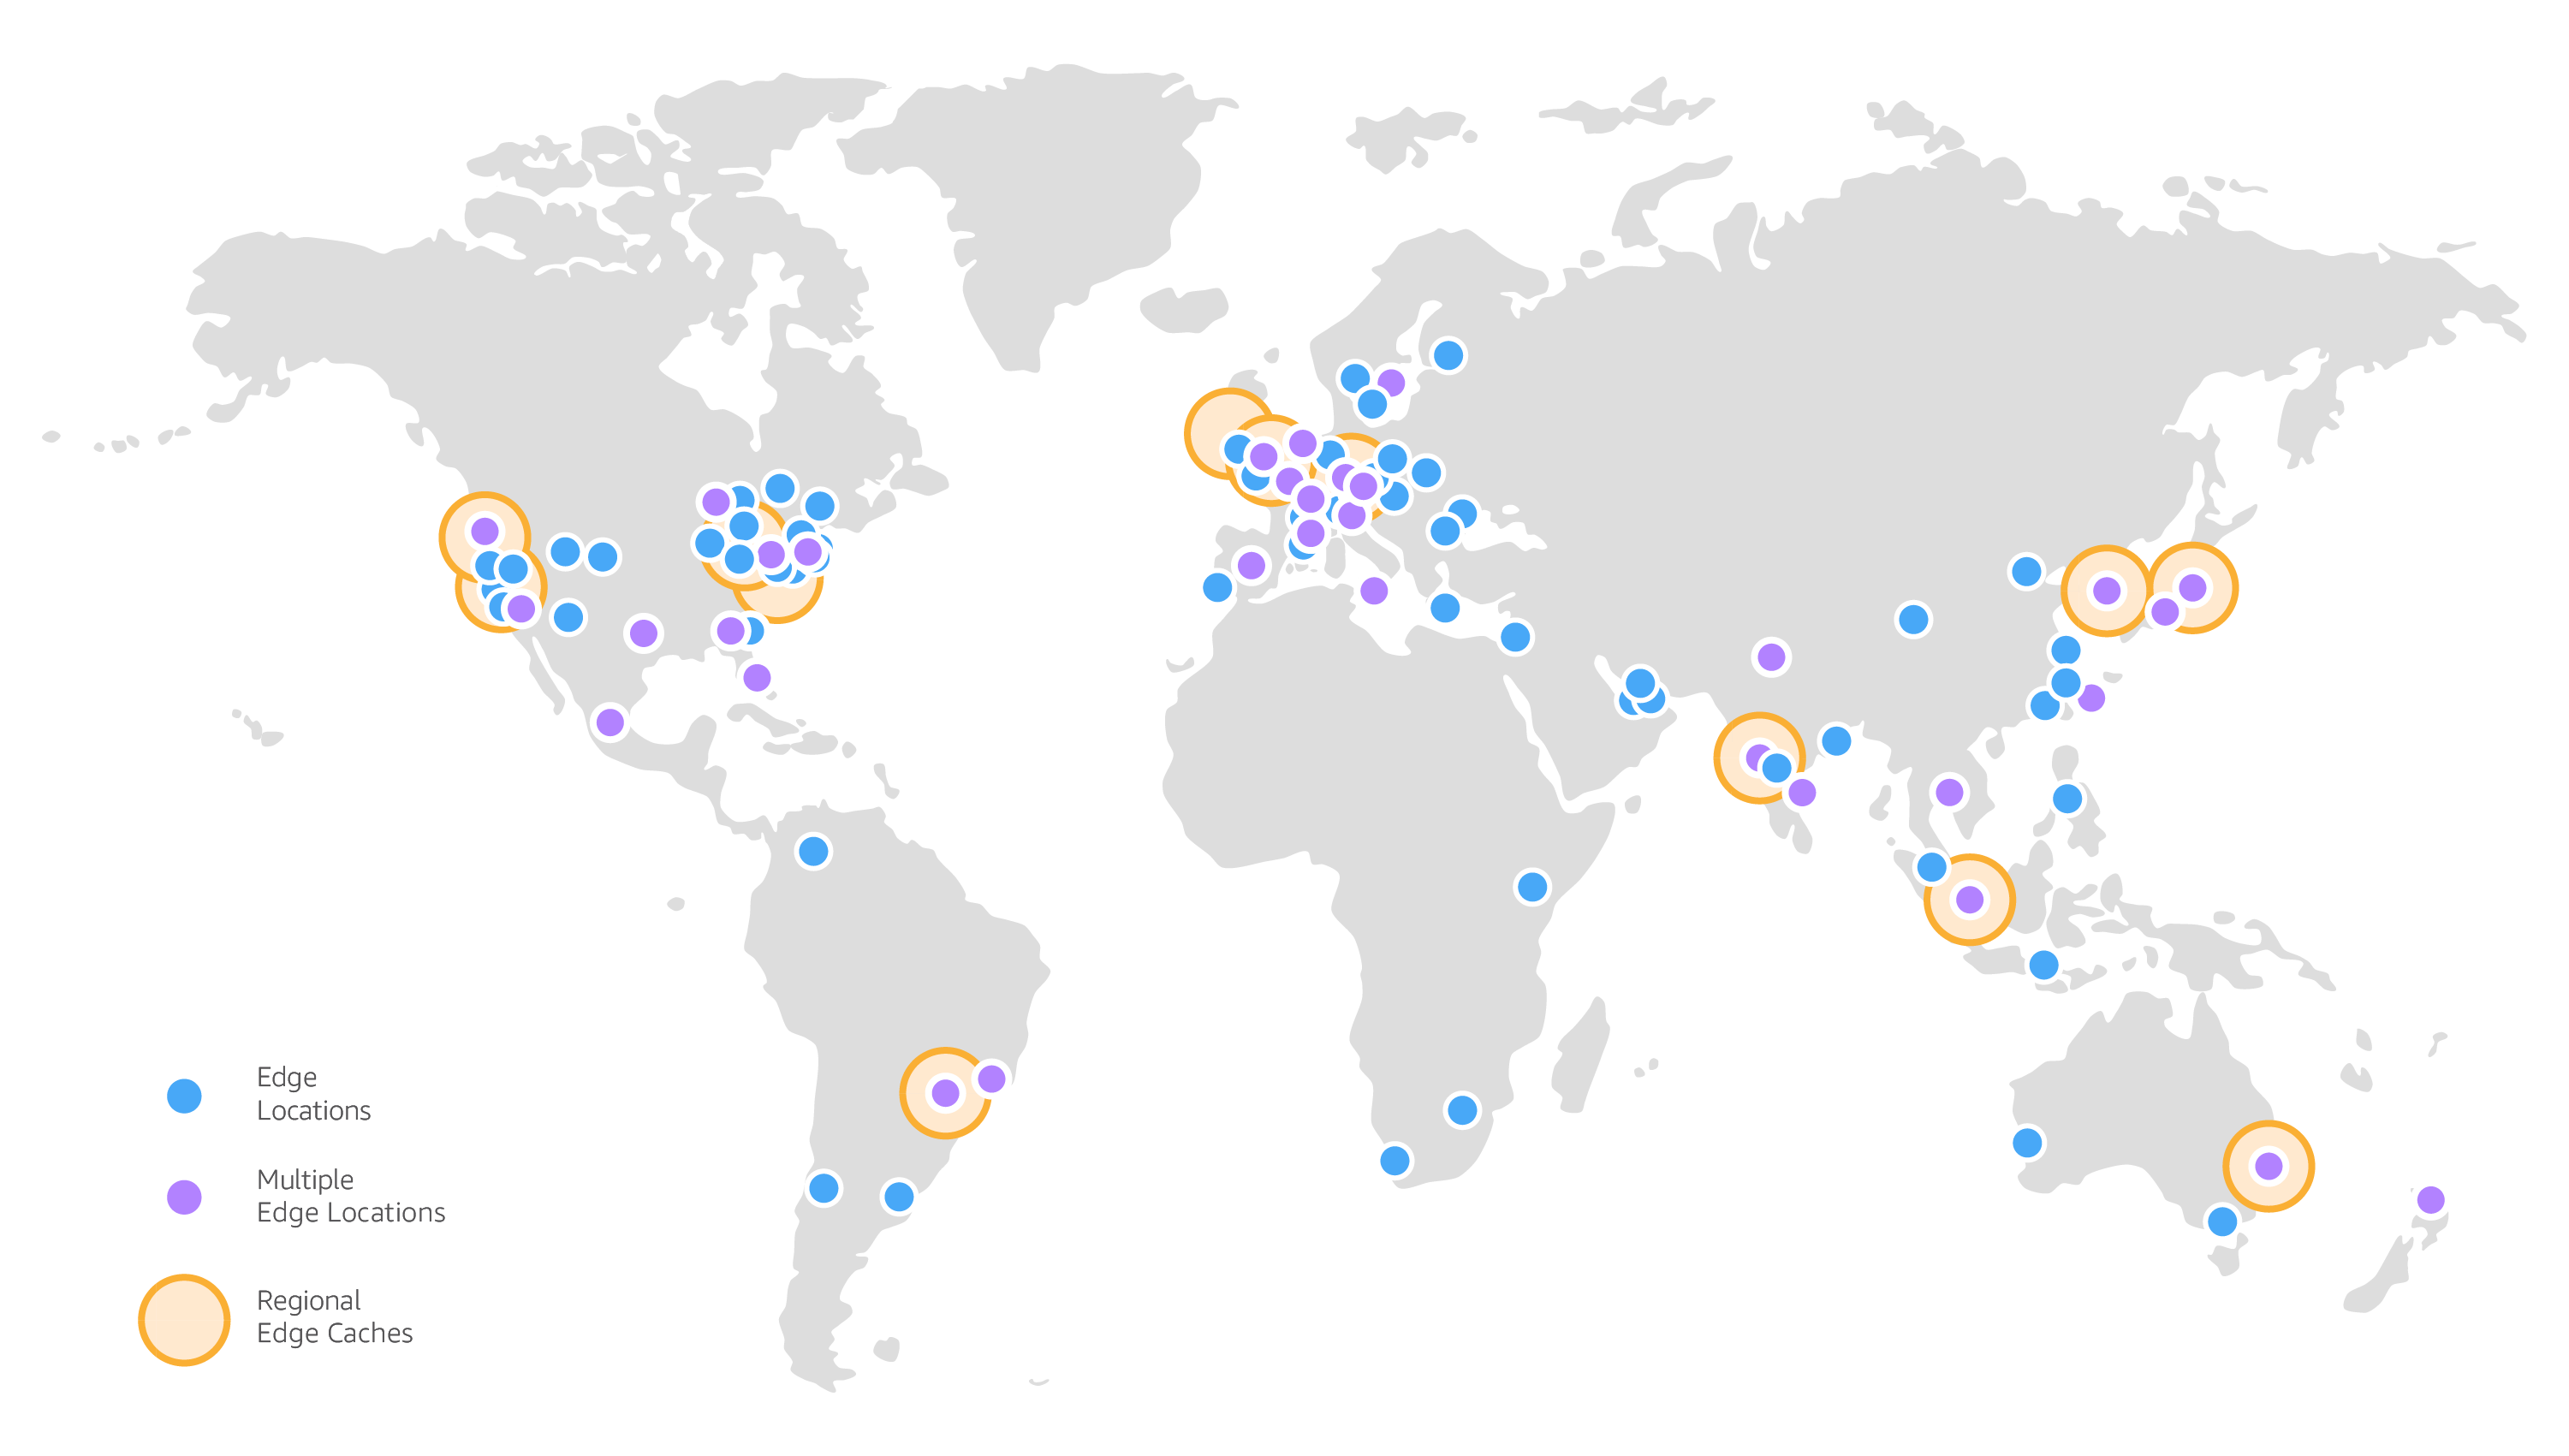
\includegraphics[scale=0.3]{Imagens/aws_zones.png}
    \legend{Fonte: \cite{ref:008}.}
    \label{fig:aws_zone}
\end{figure}

Para o desenvolvimento de aplicações na AWS, a Amazon oferece ao desenvolvedor ferramentas e permite a escolha da linguagem de programação. Destaca-se as seguintes ferramentas:

\begin{itemize}
    \item Console da web;
    \item Ferramenta de linha de comando;
    \item IDE;
    \item SDK;
    \item Infraestrutura como código.
\end{itemize}

% -----------------------------------------------------------------------------
% Capítulo 2.3 - AWS IAM
% -----------------------------------------------------------------------------
\section{AWS IAM}

O AWS IAM é um serviço da Amazon que gerencia e controla o acesso aos recursos da AWS. Com o IAM, o usuário controla de maneira centralizada quem é autenticado (conectado) e autorizado (tem permissões) para usar recursos \cite{ref:010}.

Ao criar uma conta AWS, uma identidade de login é iniciada. Essa identidade é chamada de usuário raiz da conta AWS e tem acesso completo a todos os serviços e recursos. O usuário raiz, contudo, não é recomendado em tarefas diárias. Recomenda-se que usuários tenham um privilégio mínimo e refinado para as suas tarefas.

Ademais, o IAM oferece um controle de acesso baseado em atributos, o que permite a criação de permissões baseadas em particularidades (como departamento, cidade e nome da equipe) \cite{ref:011}.

A \autoref{fig:iam_diagram} apresenta um diagrama detalhando o funcionamento do serviço AWS IAM.

\begin{figure}[htb]
    \centering
    \caption{Diagrama do serviço AWS IAM.}
    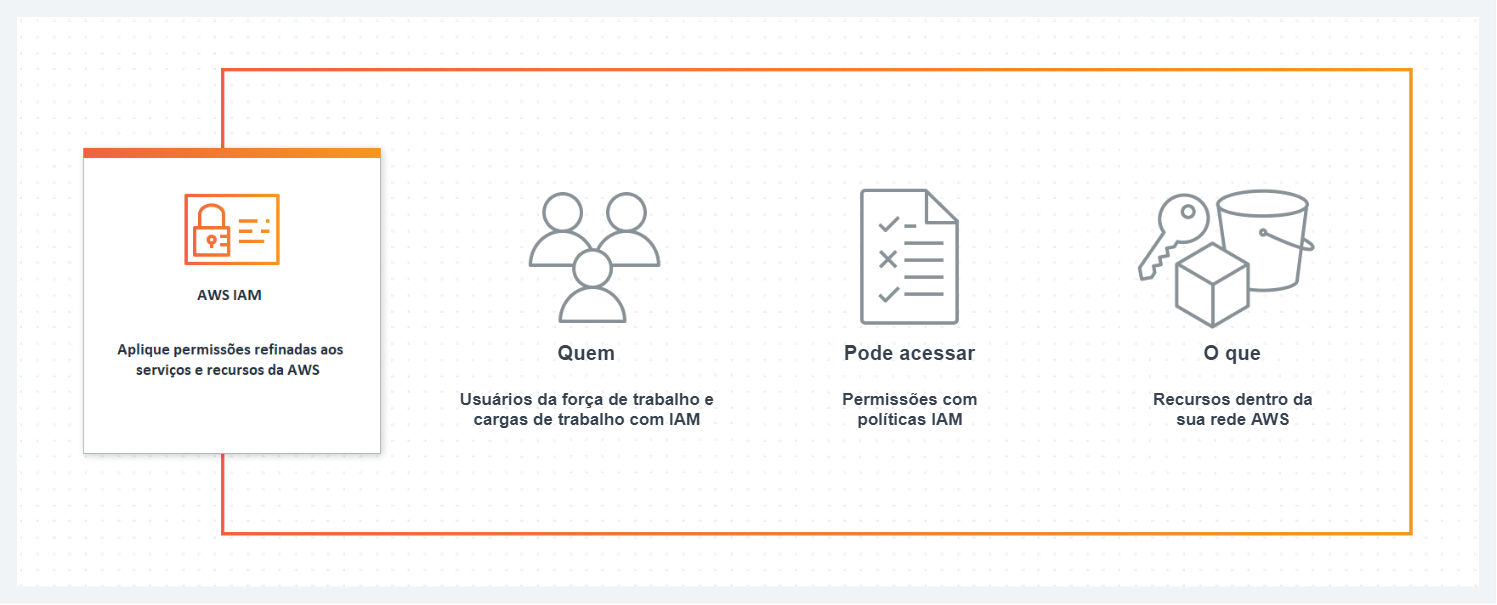
\includegraphics[scale=0.3]{Imagens/iam_diagram.png}
    \legend{Fonte: \cite{ref:011}, com edições feitas pelo autor.}
    \label{fig:iam_diagram}
\end{figure}

% -----------------------------------------------------------------------------
% Capítulo 2.4 - Segurança
% -----------------------------------------------------------------------------
\section{Segurança}\label{section:aws_iot_security}

A AWS adota um modelo de responsabilidade compartilhada de segurança e conformidade entre a AWS e o cliente. Esse modelo tem como principais conceitos o que a Amazon chama de ``segurança da nuvem'' e ``segurança na nuvem'' \cite{ref:012}.

A ``segurança da nuvem'' define que a AWS é responsável por prover serviços seguros proteger a infraestrutura que executa todos os serviços oferecidos na Nuvem AWS. Já a ``segurança na nuvem'' é definida pelo serviço da AWS que o cliente estiver usando. Por exemplo, o serviço Amazon EC2 exige que o cliente execute todas as tarefas necessárias de configuração e gerenciamento da segurança. o cliente também é responsável por fatores como a sensibilidade dos dados, os requisitos da empresa e aplicáveis leis e regulações \cite{ref:013}. A \autoref{fig:modelo_compartilhado_de_responsabilidade} mostra um diagrama oferecido pela AWS que descreve o modelo compartilhado de responsabilidade.

\begin{figure}[htbp]
    \centering
    \caption{Modelo Compartilhado de Responsabilidade de Amazon.}
    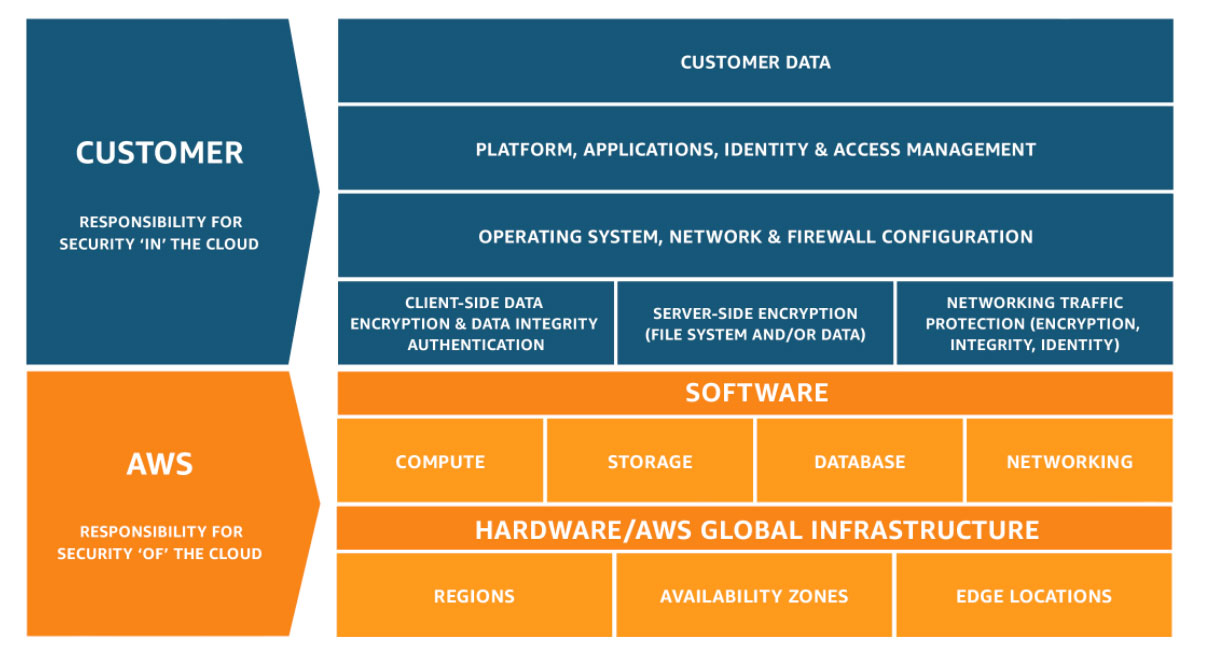
\includegraphics[scale=0.35]{Imagens/modelo_compartilhado_de_responsabilidade.jpg}
    \legend{Fonte: \cite{ref:013}.}
    \label{fig:modelo_compartilhado_de_responsabilidade}
\end{figure}

Além disso, todo tráfego de dados acontece via TLS. TLS é um protocolo criptográfico projetado para fornecer segurança da comunicação em uma rede de computadores. O protocolo é amplamente usado em aplicativos como e-mail e mensagens instantâneas, mas seu uso na proteção de HTTPS continua sendo o mais visível publicamente \cite{ref:014}.

Para o serviço AWS IoT, que será mais bem detalhado na sessão \autoref{section:aws_iot}, cada dispositivo e cliente precisa ter credenciais para a iteração com a rede IoT. O cliente é responsável por gerenciar credencias para cada dispositivo e políticas para o serviço AWS IoT. As credenciais têm o papel de criar identidade única para os dispositivos, enquanto as políticas administram as permissões de cada dispositivo ou grupo de dispositivos.

As credenciais geradas para cada dispositivo são uma forma de autenticação. Autenticação é um mecanismo de verificação de identidade de um cliente e/ou servidor \cite{ref:016}. Um exemplo de certificado é o X.509. Os certificados X.509 são certificados digitais que usam o padrão de infraestrutura de chave pública X.509 para associar uma chave pública a uma identidade contida em um certificado \cite{ref:015}. As cadeias de certificados X.509 são usadas para autenticação de servidor por clientes e autenticação de cliente pelo servidor.

As políticas, por sua vez, são mecanismos de autorização. Autorização é o processo de garantir permissões a uma identidade autenticada \cite{ref:017}. De forma simples, as políticas determinam o que uma identidade autenticada pode fazer. Considere, por exemplo, um dispositivo conectado ao serviço AWS IoT com um certificado X.509. Com um documento de política, esse dispositivo pode ter acesso a todos os tópicos MQTT ou um número restrito de tópicos.

Para o gerenciamento de políticas, a AWS faz uso de documentos no formato JSON. O \autoref{lst:iot_policy} mostra um exemplo de política que dá permissões para um dispositivo IoT acessar recursos do serviço AWS IoT de um usuário raiz com ID 332527922592 e localizado na região ``\textit{sa-east-1}'' (São Paulo).

\begin{lstlisting}[float=htbp,language=json,firstnumber=1,caption={Exemplo de uma política dando permissões de uso do serviço AWS IoT para um dispositivo IoT.},label=lst:iot_policy]
{
    "Effect": "Allow",
    "Action": "iot:Publish",
    "Resource": "arn:aws:iot:sa-east-1:332527922592:*"
},
{
    "Effect": "Allow",
    "Action": "iot:Receive",
    "Resource": "arn:aws:iot:sa-east-1:332527922592:*"
}
\end{lstlisting}

% -----------------------------------------------------------------------------
% Capítulo 2.5 AWS IoT
% -----------------------------------------------------------------------------
\section{AWS IoT}\label{section:aws_iot}

O AWS IoT é um conjunto de serviços em nuvem oferecidos pela AWS que permitem a conexão de dispositivos IoT a outros dispositivos e a outros serviços oferecidos pelo AWS. Em termos simples, o AWS IoT funciona como uma ponte entre dispositivos IoT e os serviços em nuvem que a AWS fornece, assim como pode ser visto na \autoref{fig:what_is_iot}.

\begin{figure}[htbp]
    \centering
    \caption{Integração de dispositivos IoT com serviços AWS por meio do AWS IoT.}
    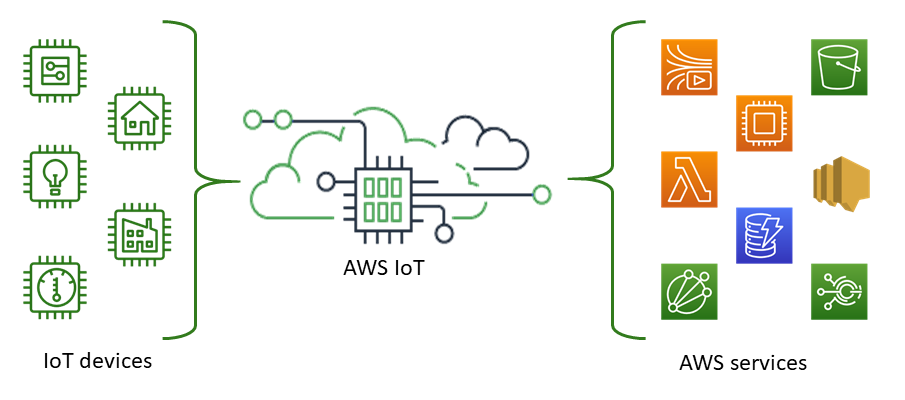
\includegraphics[scale=0.5]{Imagens/what-is-aws-iot.png}
    \legend{Fonte: \cite{ref:018}.}
    \label{fig:what_is_iot}
\end{figure}

Os dispositivos IoT geralmente estão localizados próximos às interfaces do mundo real que monitoram e/ou controlam. Eles geralmente também incluem recursos de computação e armazenamento, como microcontroladores, CPUs e memórias. Alguns exemplos de dispositivos disponíveis no mercado são \cite{ref:019}:

\begin{itemize}
    \item LoRaWAN e dispositivos;
    \item Arduino;
    \item Raspberry PI;
    \item Dispositivos de IoT personalizados.
\end{itemize}

Para a completa integração desses dispositivos com serviços AWS e usuários, alguns componentes são essenciais. Aplicativos de celulares, por exemplo, são utilizados para que o usuário tenha acesso aos seus aparelhos e os configure conforme a sua preferência \cite{ref:019}. Tem-se como outro exemplo os protocolos utilizados para a comunicação dos dispositivos com serviços em nuvem. A tecnologia AWS IoT possui suporte para os seguintes protocolos:

\begin{itemize}
    \item MQTT;
    \item HTTPS;
    \item LoRaWAN.
\end{itemize}

O protocolo MQTT será mais bem detalhado na sessão \autoref{section:mqtt}. Para o desenvolvimento de softwares a nível de dispositivo, o AWS IoT também fornece suporte para um sistema operacional em tempo real para microcontroladores, o FreeRTOS. Alguns exemplos de outros serviços que o AWS IoT oferece suporte podem ser vistos na \autoref{fig:aws_iot_architecture}.

\begin{figure}[htbp]
    \centering
    \caption{Exemplos de serviços fornecidos pelo AWS IoT.}
    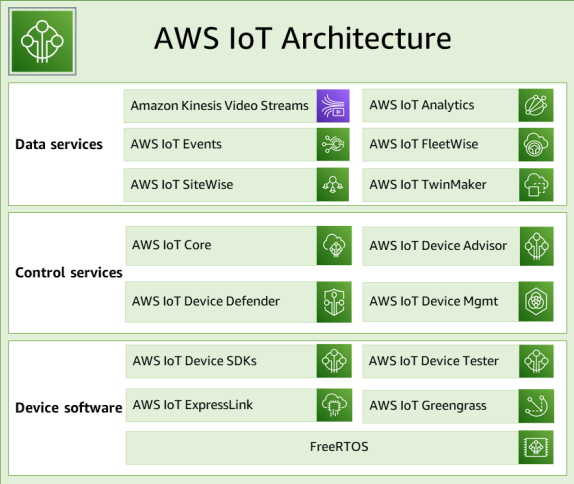
\includegraphics[scale=0.7]{Imagens/aws_iot_architecture.png}
    \legend{Fonte: \cite{ref:019}.}
    \label{fig:aws_iot_architecture}
\end{figure}

O serviço IoT Core será mais bem detalhado na sessão \autoref{subsection:aws_iot_core}.

% ------------------------------------------------------------------------------------------------
% Capítulo 2.5.1 - AWS IoT Core
% -----------------------------------------------------------------------------
\subsection{AWS IoT Core}\label{subsection:aws_iot_core}

O AWS IoT Core é serviço de controle oferecido pela AWS que permite a conexão de bilhões de dispositivos de IoT e rotear trilhões de mensagens para serviços da AWS sem que o usuário tenha que gerenciar a infraestrutura \cite{ref:020}. Esse serviço está disponível gratuitamente para clientes por doze meses a partir da data em que a conta da AWS é criada. Haverá taxas de uso do AWS IoT core após doze meses de uso ou quando a aplicação exceder os níveis de uso gratuito descritos abaixo \cite{ref:021}:

\begin{itemize}
    \item 2.250.000 minutos de conexão;
    \item 500.000 mensagens;
    \item 225.000 operações do Registry ou Device Shadow;
    \item 250.000 regras acionadas e 250.000 ações executadas.
\end{itemize}

Dessa forma, o AWS IoT Core é o serviço que permite a gerência de dispositivos inteligentes. A comunicação do serviço AWS IoT com os nós da rede IoT acontece via protocolo MQTT. Os preços cobrados pela AWS após doze meses de uso ou excedendo os limites já citados pode ser visto abaixo \cite{ref:021}:

\begin{itemize}
    \item Preço da conectividade: 0,12 USD (por milhão de minutos de conexão);
    \item Até 1 bilhão de mensagens MQTT e HTTP: 1,50 USD (por milhão de mensagens);
    \item Próximos 4 bilhões de mensagens MQTT e HTTP: 1,20 USD (por milhão de mensagens);
    \item Mais de 5 bilhões de mensagens MQTT e HTTP: 1,05 USD (por milhão de mensagens).
\end{itemize}

% -----------------------------------------------------------------------------
% Capítulo 2.6 - AWS Lambda
% -----------------------------------------------------------------------------
\section{AWS Lambda}\label{section:aws_lambda}

O AWS Lambda é um serviço que permite a execução de códigos sem que o usuário se preocupe com infraestrutura. A computação ocorre sem servidor e é orientado a eventos \cite{ref:022}. Esses eventos podem ser mudanças de estado ou atualizações, como por exemplo o usuário acionando alguma tarefa através da Alexa. O AWS Lambda permite, também, que o usuário estenda a lógica de outros serviços da AWS. Sumariamente, o serviço AWS Lambda permite que o usuário execute serviços de back-end sem provisionar ou gerenciar servidores.

O nível gratuito do AWS Lambda inclui um milhão de solicitações gratuitas por mês e 400.000 GB-segundos de tempo de computação por mês. Caso esses limites sejam excedidos, a precificação acontece sobre o número total de solicitações feitas por todas as funções. O preço final depende da quantidade de memória alocada por função \cite{ref:023}.

Para começar a usar o AWS Lambda, o usuário deve primeiro carregar o código na nuvem AWS. Isso pode ser feito via AWS CLI, submissão de um arquivo no formato zip ou até mesmo criando o código diretamente no console do Lambda.  O Lambda oferece suporte nativo às linguagens Java, Go, PowerShell, Node.js, C\#, Python e Ruby \cite{ref:024}. Após o carregamento do código, o usuário deve também configurar a memória e o tempo limites da função. Além disso, o usuário deve especificar o recurso que acionará a função. Alguns exemplos de recursos acionadores são uma transmissão do Amazon Kinesis e um evento gerado pela Alexa.

A \autoref{fig:exemplo_aws_lambda} mostra um exemplo de uso do AWS Lambda. Nesse exemplo, a Alexa gera um evento acionador e a função transmite mensagens via tópicos MQTT para o AWS IoT.

\begin{figure}[htbp]
    \centering
    \caption{Exemplos de uso do AWS Lambda com a Alexa gerando um evento acionador.}
    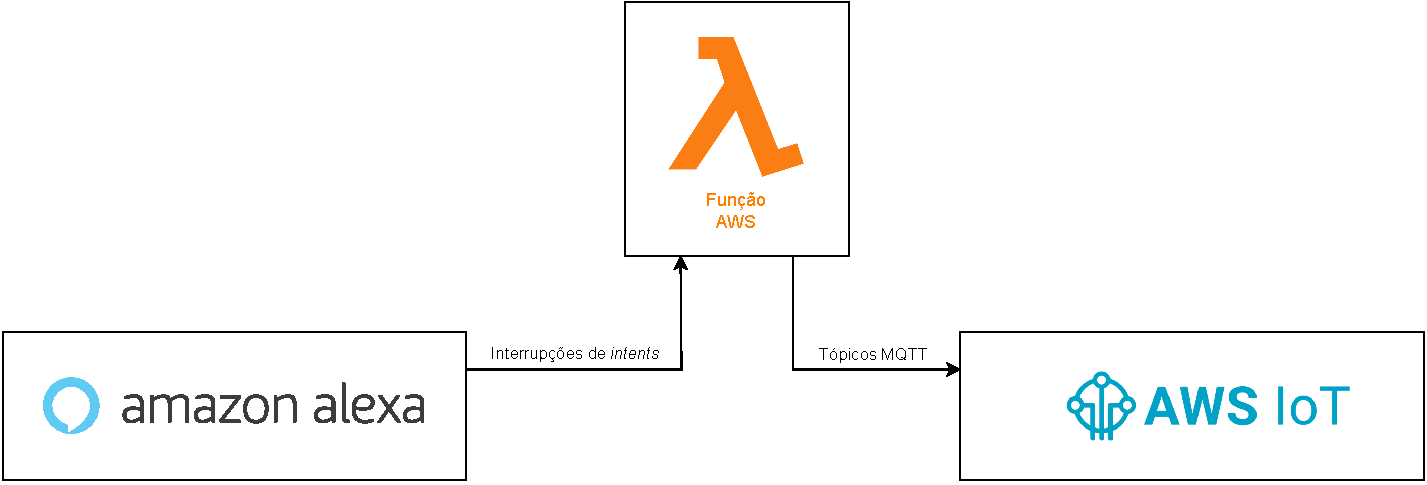
\includegraphics[scale=0.6]{Imagens/exemplo_aws_lambda.pdf}
    \legend{Fonte: Produzido pelo autor (2022).}
    \label{fig:exemplo_aws_lambda}
\end{figure}

% -----------------------------------------------------------------------------
% Capítulo 2.7 - MQTT
% -----------------------------------------------------------------------------
\section{MQTT}\label{section:mqtt}

MQTT é um protocolo de mensagens para dispositivos IoT. Ele foi desenvolvido para dispositivos com limitada disponibilidade de largura de banda (\textit{network bandwidth}). Ele deve ser executado em um protocolo de transporte que forneça conexões bidirecionais ordenadas, sem perdas - normalmente, TCP/IP \cite{ref:025}.

No protocolo MQTT, existem dois tipos de entidades: o \textit{message broker} e os clientes. Um \textit{message broker} é um servidor que tem o papel de receber diversas mensagens dos diversos clientes e, então, as rotear para os clientes de destino. Já um cliente pode ser qualquer dispositivo que se comunica via rede com o \textit{message broker}, a partir de bibliotecas do protocolo MQTT \cite{ref:025}.

As informações são organizadas em hierarquia de tópicos. Quando algum cliente possui um novo item de dados para distribuir, ele envia uma mensagem de controle com os dados para o \textit{message broker}. O \textit{broker}, então, distribui as informações para todos os clientes que se inscreveram nesse tópico. O cliente remetente (\textit{publisher}) não precisa ter nenhuma informação sobre número de clientes que irão receber essa mensagem. Os clientes destinatários, por sua vez, também não precisam ser configurados com nenhuma informação dos destinatários.

Os sete tipos de mensagens existentes no protocolo MQTT são \cite{ref:025}:

\begin{itemize}
    \item \textit{Connect}: Aguarda o estabelecimento de uma conexão com o \textit{message broker} e cria um link entre os nós;
    \item \textit{Disconnect}: Aguarda o fim da tarefa que está sendo executada pelo cliente e desconecta a sessão TCP/IP;
    \item \textit{Publish}: Mensagem a ser distribuída para os clientes inscritos. Mais informações sobre esse tipo de mensagem podem ser encontrado na \autoref{subsection:mqtt_publish_message}.
    \item \textit{Subscribe}: Para receber mensagens sobre tópicos de interesse, o cliente envia uma mensagem \textit{Subscribe} para o \textit{broker}. Mais informações sobre esse tipo de mensagem podem ser encontrado na \autoref{subsection:mqtt_subscribe_message};
    \item \textit{Suback}: Para confirmar cada assinatura, o \textit{broker} envia uma mensagem de confirmação \textit{Suback} ao cliente. Mais informações sobre esse tipo de mensagem podem ser encontrado na \autoref{subsection:mqtt_subscribe_message};
    \item \textit{Unsubscribe}: Esta mensagem exclui as assinaturas existentes de um cliente no \textit{broker}. Mais informações sobre esse tipo de mensagem podem ser encontrado na \autoref{subsection:mqtt_unsubscribe_message};
    \item \textit{Unsuback}: Para confirmar o cancelamento de assinatura, o \textit{broker} envia uma mensagem de confirmação \textit{Unsuback} ao cliente. Mais informações sobre esse tipo de mensagem podem ser encontrado na \autoref{subsection:mqtt_unsuback_message}.
\end{itemize}

Depois que um cliente envia com êxito a mensagem \textit{Subscribe} e recebe a mensagem \textit{Suback}, ele obtém todas as mensagens publicadas de um tópico nas assinaturas contidas da mensagem \textit{Subscribe}. Após receber o \textit{Unsuback} do \textit{broker}, o cliente pode assumir que as assinaturas na mensagem \textit{Unsubscribe} foram excluídas.

Se o \textit{message broker} receber uma mensagem em um tópico para o qual não há assinantes, a mensagem será descartada. Quando um cliente \textit{publisher} se conecta pela primeira vez ao \textit{broker}, ele pode configurar uma mensagem padrão para ser enviada aos assinantes se o \textit{broker} detectar que o cliente \textit{publisher} se desconectou inesperadamente.

Os clientes interagem apenas com um \textit{broker}, mas um sistema pode conter vários \textit{brokers} que trocam informações com base nos tópicos de seus assinantes atuais. Uma mensagem de controle MQTT deve ter entre dois e duzentos e cinquenta e seis bytes. O MQTT conta com o protocolo TCP para transmissão de dados. Uma variante, MQTT-SN, é usada com outros protocolos de transporte, como UDP ou Bluetooth.

A \autoref{fig:rede_mqtt} mostra um exemplo de uma rede MQTT com quatro clientes.

\begin{figure}[htbp]
    \centering
    \caption{Exemplo de uma rede MQTT com quatro clientes.}
    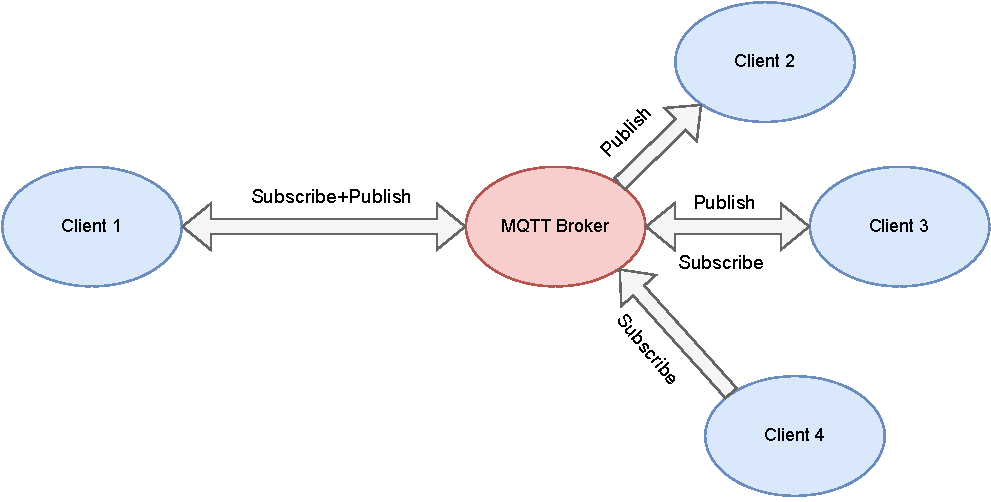
\includegraphics[scale=0.7]{Imagens/mqtt_protocol.pdf}
    \legend{Fonte: Produzido pelo autor (2022).}
    \label{fig:rede_mqtt}
\end{figure}

% -----------------------------------------------------------------------------
% Capítulo 2.5.1 - MQTT Publish Message
% -----------------------------------------------------------------------------
\subsection{MQTT Publish Message}\label{subsection:mqtt_publish_message}

O formato de uma mensagem do tipo \textit{Publish} está apresentado na \autoref{fig:mqtt_publish_message_attributes}.

\begin{figure}[htbp]
    \centering
    \caption{Atributos de uma mensagem do tipo \textit{Publish} para o protocolo MQTT.}
    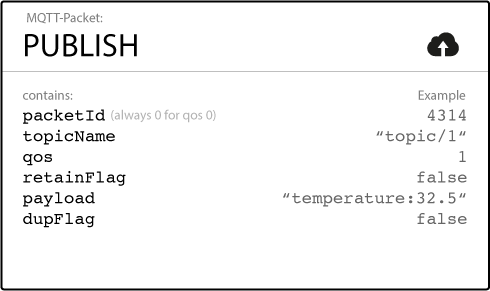
\includegraphics[scale=0.5]{Imagens/mqtt_publish_message_attributes.png}
    \legend{Fonte: \cite{ref:026}.}
    \label{fig:mqtt_publish_message_attributes}
\end{figure}

Os atributos de uma mensagem do tipo \textit{Publish} são caracterizados abaixo \cite{ref:026}:

\begin{itemize}
    \item packetId: O identificador de pacote identifica exclusivamente uma mensagem;
    \item topicName: O nome do tópico é uma \textit{string} simples que é estruturada hierarquicamente com barras como delimitadores (``alexa/builtin/device'', por exemplo);
    \item qos: Indica o nível de qualidade de serviço (QoS) da mensagem. Existem três níveis: 0, 1 e 2. O nível de serviço determina que tipo de garantia uma mensagem tem para chegar ao destinatário pretendido (cliente ou \textit{broker}).
    \item retainFlag: Sinalizador indicando se a mensagem é salva pelo \textit{broker} como o último valor válido conhecido para um tópico especificado. Quando um novo cliente se inscreve em um tópico, ele recebe a última mensagem retida nesse tópico.
    \item payLoad: Conteúdo da mensagem. O MQTT é \textit{data-agnostic}. Ou seja, é possível enviar qualquer tipo de informação que pode ser codificada em formato binário.
    \item dupFlag: Indica se a mensagem é uma duplicata e foi reenviada porque o destinatário pretendido (cliente ou \textit{broker}) não enviou uma resposta de \textit{acknowledge}.
\end{itemize}

% -----------------------------------------------------------------------------
% Capítulo 2.5.2 - MQTT Subscribe Message
% -----------------------------------------------------------------------------
\subsection{MQTT Subscribe Message}\label{subsection:mqtt_subscribe_message}

O formato de uma mensagem do tipo \textit{Subscribe} está apresentado na \autoref{fig:mqtt_subscribe_message_attributes}. Esta mensagem de assinatura é muito simples, contém um identificador de pacote exclusivo e uma lista de assinaturas.

\begin{figure}[htbp]
    \centering
    \caption{Atributos de uma mensagem do tipo \textit{Subscribe} para o protocolo MQTT.}
    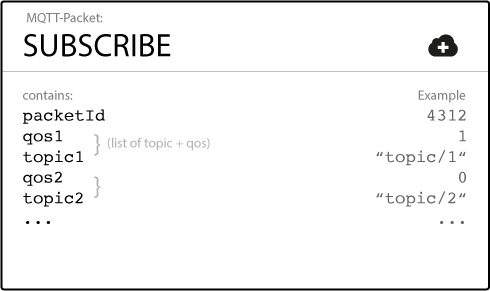
\includegraphics[scale=0.5]{Imagens/mqtt_subscribe_message_attributes.png}
    \legend{Fonte: \cite{ref:026}.}
    \label{fig:mqtt_subscribe_message_attributes}
\end{figure}

Os atributos de uma mensagem do tipo \textit{Subscribe} são caracterizados abaixo \cite{ref:026}:

\begin{itemize}
    \item packetId: O identificador de pacote identifica exclusivamente uma mensagem;
    \item \textit{List of Subscriptions}: Uma mensagem \textit{Subscribe} pode conter várias assinaturas para um cliente. Cada assinatura é composta por um tópico (\textit{topici}) e um nível de QoS (\textit{qosi}). O tópico pode conter \textit{wildcards} que possibilitam a assinatura de um padrão de tópicos em vez de um tópico específico. Se houver assinaturas sobrepostas para um cliente, o \textit{broker} entrega a mensagem que possui o nível de QoS mais alto para esse tópico.
\end{itemize}

% -----------------------------------------------------------------------------
% Capítulo 2.5.3 - MQTT Suback Message
% -----------------------------------------------------------------------------
\subsection{MQTT Suback Message}\label{subsection:mqtt_suback_message}

O formato de uma mensagem do tipo \textit{Suback} está apresentado na \autoref{fig:mqtt_suback_message_attributes}. Esta mensagem contém o identificador de pacote da mensagem \textit{Subscribe} original e uma lista de códigos de retorno.

\begin{figure}[htbp]
    \centering
    \caption{Atributos de uma mensagem do tipo \textit{Suback} para o protocolo MQTT.}
    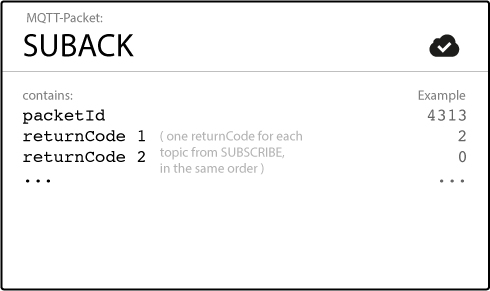
\includegraphics[scale=0.5]{Imagens/mqtt_suback_message_attributes.png}
    \legend{Fonte: \cite{ref:026}.}
    \label{fig:mqtt_suback_message_attributes}
\end{figure}

Os atributos de uma mensagem do tipo \textit{Suback} são caracterizados abaixo \cite{ref:026}:

\begin{itemize}
    \item packetId: O identificador de pacote identifica exclusivamente uma mensagem;
    \item \textit{Return Code}: O \textit{broker} envia um código de retorno para cada par de tópico/QoS que recebe de mensagens \textit{Subscribe}. O código de retorno reconhece cada tópico e mostra o nível de QoS concedido pelo \textit{broker}. Se o \textit{broker} recusar uma assinatura, a mensagem \textit{Suback} conterá um código de retorno de falha para esse tópico específico.
\end{itemize}

% -----------------------------------------------------------------------------
% Capítulo 2.5.4 - MQTT Unsubscribe Message
% -----------------------------------------------------------------------------
\subsection{MQTT Unsubscribe Message}\label{subsection:mqtt_unsubscribe_message}

O formato de uma mensagem do tipo \textit{Unsubscribe} está apresentado na \autoref{fig:mqtt_unsubscribe_message_attributes}. A mensagem \textit{Unsubscribe} é semelhante à mensagem  \textit{Subscribe} e possui um identificador de pacote e uma lista de tópicos.

\begin{figure}[htbp]
    \centering
    \caption{Atributos de uma mensagem do tipo \textit{Unsubscribe} para o protocolo MQTT.}
    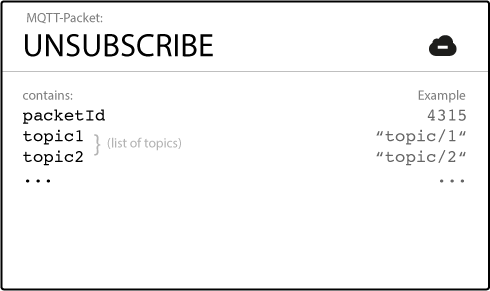
\includegraphics[scale=0.5]{Imagens/mqtt_unsubscribe_message_attributes.png}
    \legend{Fonte: \cite{ref:026}.}
    \label{fig:mqtt_unsubscribe_message_attributes}
\end{figure}

Os atributos de uma mensagem do tipo \textit{Unsubscribe} são caracterizados abaixo \cite{ref:026}:

\begin{itemize}
    \item packetId: O identificador de pacote identifica exclusivamente uma mensagem;
    \item \textit{List of Topic}: A lista de tópicos pode conter vários tópicos dos quais o cliente deseja cancelar a assinatura. Só é necessário enviar o tópico (sem QoS). O \textit{broker} cancela a assinatura do tópico, independentemente do nível de QoS com o qual foi originalmente assinado.
\end{itemize}

% -----------------------------------------------------------------------------
% Capítulo 2.5.5 - MQTT Unsuback Message
% -----------------------------------------------------------------------------
\subsection{MQTT Unsuback Message}\label{subsection:mqtt_unsuback_message}

O formato de uma mensagem do tipo \textit{Unsuback} está apresentado na \autoref{fig:mqtt_unsuback_message_attributes}. Esta mensagem contém apenas o identificador de pacote da mensagem \textit{Unsubscribe} original.

\begin{figure}[htbp]
    \centering
    \caption{Atributos de uma mensagem do tipo \textit{Unsuback} para o protocolo MQTT.}
    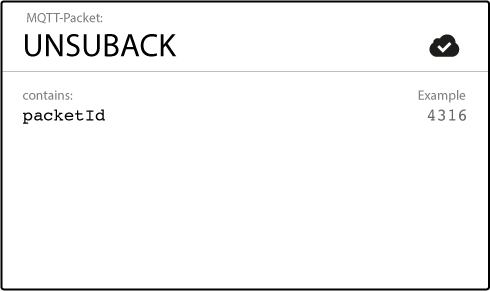
\includegraphics[scale=0.5]{Imagens/mqtt_unsuback_message_attributes.png}
    \legend{Fonte: \cite{ref:026}.}
    \label{fig:mqtt_unsuback_message_attributes}
\end{figure}

% -----------------------------------------------------------------------------
% Capítulo 2.6 - Amazon Alexa
% -----------------------------------------------------------------------------
\section{Amazon Alexa}\label{section:amazon_alexa}

A Amazon Alexa, conhecida simplesmente como Alexa, é uma assistente virtual inteligente capaz de controlar dispositivos inteligentes e ter iterações de voz com os usuários. As capacidades da Alexa podem ser expandidas por terceiros através da instalação de habilidades (aplicativos). Algumas categorias de habilidades em destaque são: Notícias, Negócios e Finanças, Jogos e Curiosidades, Saúde e Boa Forma e Produtividade \cite{ref:002}. A loja oficial de habilidades da Amazon permite que o usuário faça busca de habilidades por categorias, assim como pode ser visto na \autoref{fig:alexa_skills_categorias}.

\begin{figure}[htbp]
    \centering
    \caption{Busca de habilidades da Alexa por categorias.}
    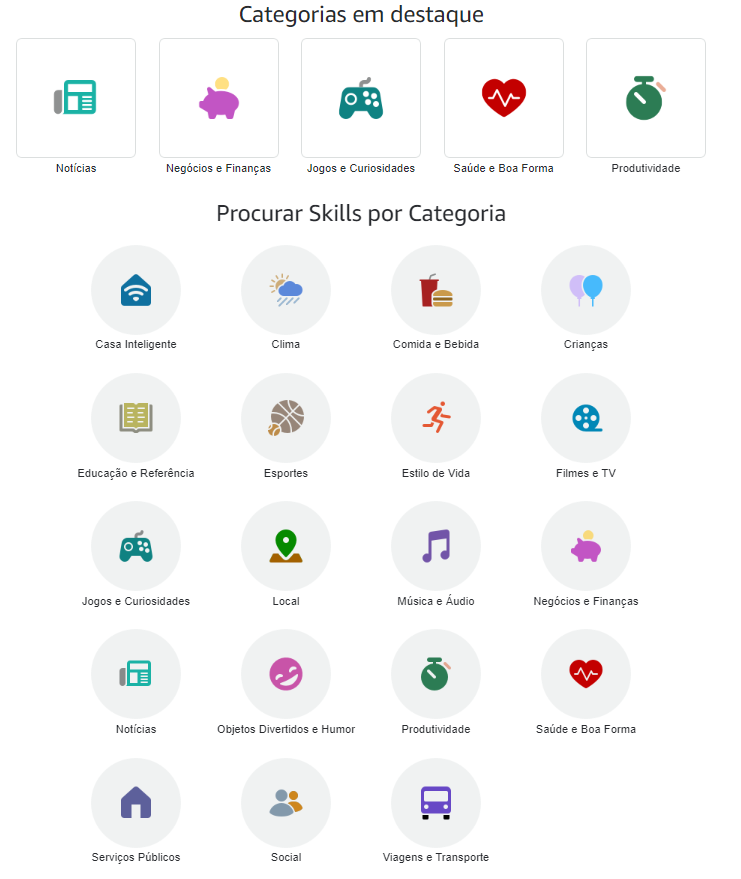
\includegraphics[scale=0.8]{Imagens/alexa_skills_categorias.png}
    \legend{Fonte: \cite{ref:028}.}
    \label{fig:alexa_skills_categorias}
\end{figure}

\subsection{Alexa Skills Kit}\label{subsection:alexa_skills_kit}
O ASK fornece APIs e ferramentas para a criação de habilidades Alexa. Empresas podem desenvolver habilidades para seus produtos e serviços, ou contratarem uma agência especialista em Alexa. Uma habilidade Alexa tem tanto uma interface de voz com o usuário, como uma lógica de aplicativo \cite{ref:029}.

Quando um usuário interage com um dispositivo Alexa, ocorre um processamento da fala no contexto do seu modelo de interação para interpretar o que foi requisitado. A Alexa, então, envia a solicitação à sua lógica de aplicação, responsável por processar e computar essa informação \cite{ref:029}. Essa computação acontece em nuvem AWS ou outro servidor. Dessa forma, caracteriza-se o processamento da fala e interpretação do que foi requisitado como front-end e a computação da lógica de aplicação como back-end. A \autoref{fig:diagrama_habilidades_alexa} mostra um diagrama produzido pela Amazon explicando o funcionamento de uma habilidade Alexa.

\begin{figure}[htbp]
    \centering
    \caption{Diagrama explicando o funcionamento de uma habilidade Alexa.}
    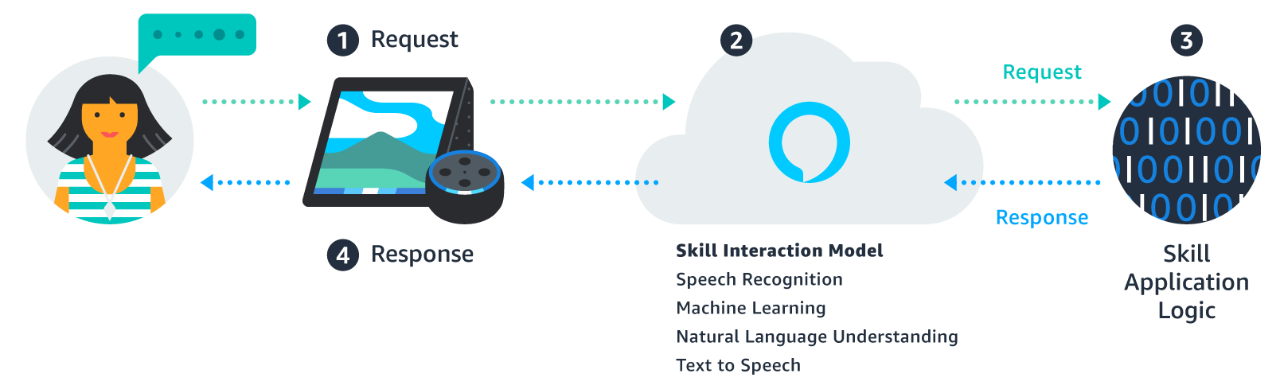
\includegraphics[scale=0.35]{Imagens/diagrama_habilidades_alexa.png}
    \legend{Fonte: \cite{ref:029}.}
    \label{fig:diagrama_habilidades_alexa}
\end{figure}

Para o desenvolvimento de software, os ASK SDKs permitem uma redução da complexidade do projeto. Os SDKs para Java, Node.js e Python fornecem funções específicas da linguagem para tarefas comuns, permitindo a concentração na lógica das habilidades, não no código padrão \cite{ref:029}. A Amazon também fornece distintas de ferramentas de desenvolvimento. O desenvolvedor pode usar o console do portal ou CLI do ASK para criar, gerenciar, testar e publicar habilidades.

\subsection{Alexa Voice Service}\label{subsection:alexa_voice_service}

A Amazon permite que fabricantes construam dispositivos com a Alexa integrada usando o AVS, um serviço baseado na AWS com APIs que permitem a integração de dispositivos com a Alexa. Dessa forma, produtos usuários do AVS têm acesso a diversos recursos da Alexa, incluindo as habilidades Alexa. A principal vantagem do AVS é o fornecimento de APIs que permitem o reconhecimento automático de fala, com computação executada em nuvem, e compreensão de linguagem natural \cite{ref:002}.

Um exemplo de uso do AVS é um dispositivo IoT com a Alexa embutida. Nesse exemplo, o desenvolvedor fará uso dos serviços AVS, AWS IoT e Login da Amazon. Um diagrama desenvolvido pela Amazon mostrando um exemplo de integração do AVS ao AWS IoT pode ser visto na \autoref{fig:integracao_avs_aws_iot}.

\begin{figure}[htbp]
    \centering
    \caption{Diagrama de integração do AVS ao serviço AWS IoT Core.}
    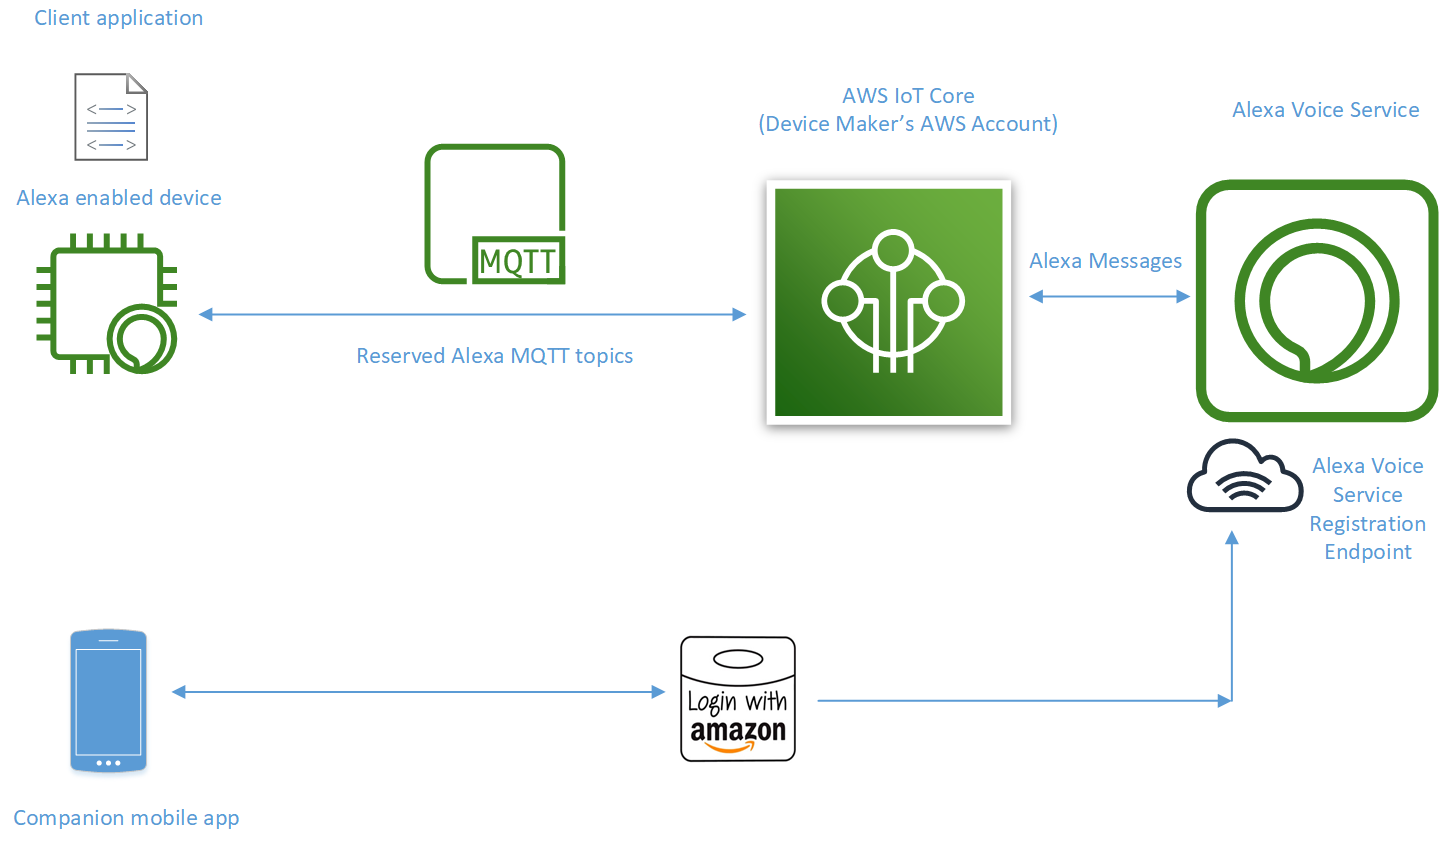
\includegraphics[scale=0.6]{Imagens/integracao_avs_aws_iot.png}
    \legend{Fonte: \cite{ref:030}.}
    \label{fig:integracao_avs_aws_iot}
\end{figure}

% -----------------------------------------------------------------------------
% Capítulo 2.6 - Trabalhos Correlatos
% -----------------------------------------------------------------------------
\section{Trabalhos correlatos}

Essa sessão busca detalhar dois trabalhos correlatos ao protótipo desse trabalho. Os dois trabalhos escolhidos são:

\begin{itemize}
    \item PROTÓTIPO DE AUTOMAÇÃO RESIDENCIAL UTILIZANDO UMA ASSISTENTE DE VOZ, de Leandro Dallarosa Neto;
    \item \textit{Creating an Alexa voice controlled IoT using a Raspberry Pi}, de John Allwork;
\end{itemize}

% -----------------------------------------------------------------------------
% Capítulo 2.6.1 - PROTÓTIPO DE AUTOMAÇÃO RESIDENCIAL UTILIZANDO UMA ASSISTENTE DE VOZ
% -----------------------------------------------------------------------------
\subsection{PROTÓTIPO DE AUTOMAÇÃO RESIDENCIAL UTILIZANDO UMA ASSISTENTE DE VOZ}\label{subsection:prototipo_de_automacao_residencial_utilizando_uma_assistente_de_voz}

Esse projeto foi desenvolvido como um Trabalho de Conclusão de Curso do aluno Leandro Dallarosa Neto, pela Universidade Regional de Blumenau \cite{ref:031}. Em resumo, o projeto teve como escopo a criação de um protótipo de automação residencial por comandos de voz utilizando a assistente pessoal Alexa. O protótipo desenvolvido utilizava o microcontrolador Arduino Ameba para controlar luzes, abrir uma porta magnética e enviar dados de temperatura para o servidor HTTP Thingspeak (2018). A computação do projeto foi feita via serviços em nuvem da AWS: o AWS Iot e o AWS Lambda. A execução do protótipo acontece por comandos de voz recebidos em um aplicativo de dispositivos móveis.

Para testes com o protótipo, uma maquete e um circuito foram montado. Esse circuito conta com o microcontrolador Arduino Ameba, dois módulos relé para Arduino, um regulador de tensão, um eletroímã de 12V e o sensor de temperatura DHT11. A \autoref{fig:circuito_eletronico_leandro_dallarosa} mostra o circuito eletrônico completo da maquete, enquanto a \autoref{fig:maquete_leandro_dallarosa} mostra a vista frontal da maquete.

\begin{figure}[htbp]
    \centering
    \caption{Circuito eletrônico completo da maquete do projeto ``PROTÓTIPO DE AUTOMAÇÃO RESIDENCIAL UTILIZANDO UMA ASSISTENTE DE VOZ''.}
    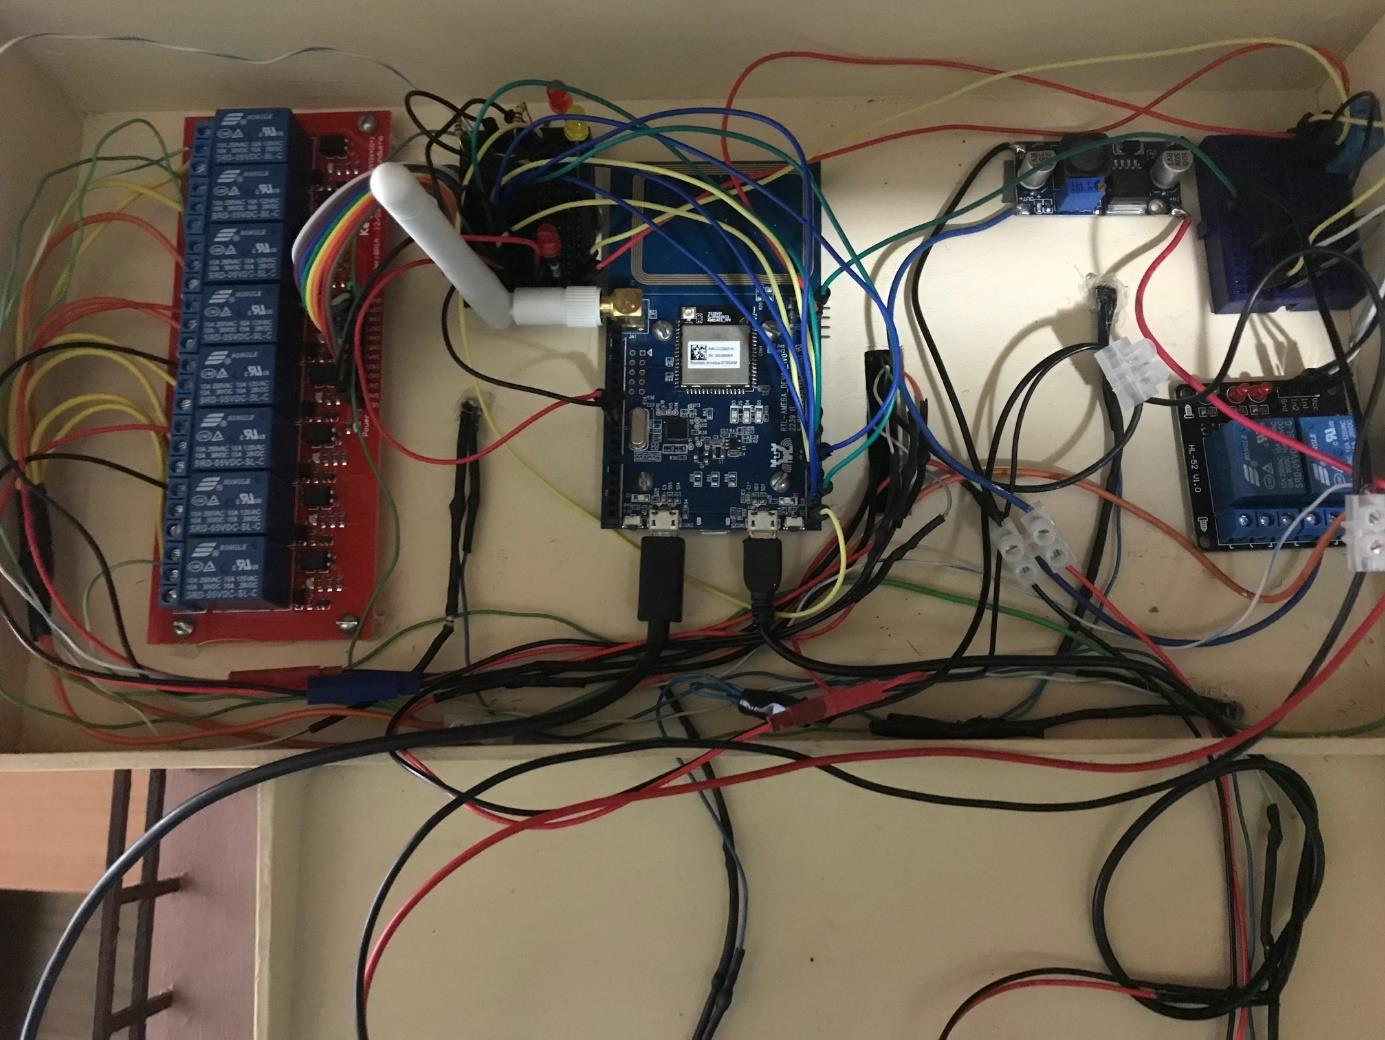
\includegraphics[scale=0.4]{Imagens/circuito_eletronico_leandro_dallarosa.png}
    \legend{Fonte: \cite{ref:031}.}
    \label{fig:circuito_eletronico_leandro_dallarosa}
\end{figure}

\begin{figure}[htbp]
    \centering
    \caption{Imagem frontal da maquete do projeto ``PROTÓTIPO DE AUTOMAÇÃO RESIDENCIAL UTILIZANDO UMA ASSISTENTE DE VOZ''.}
    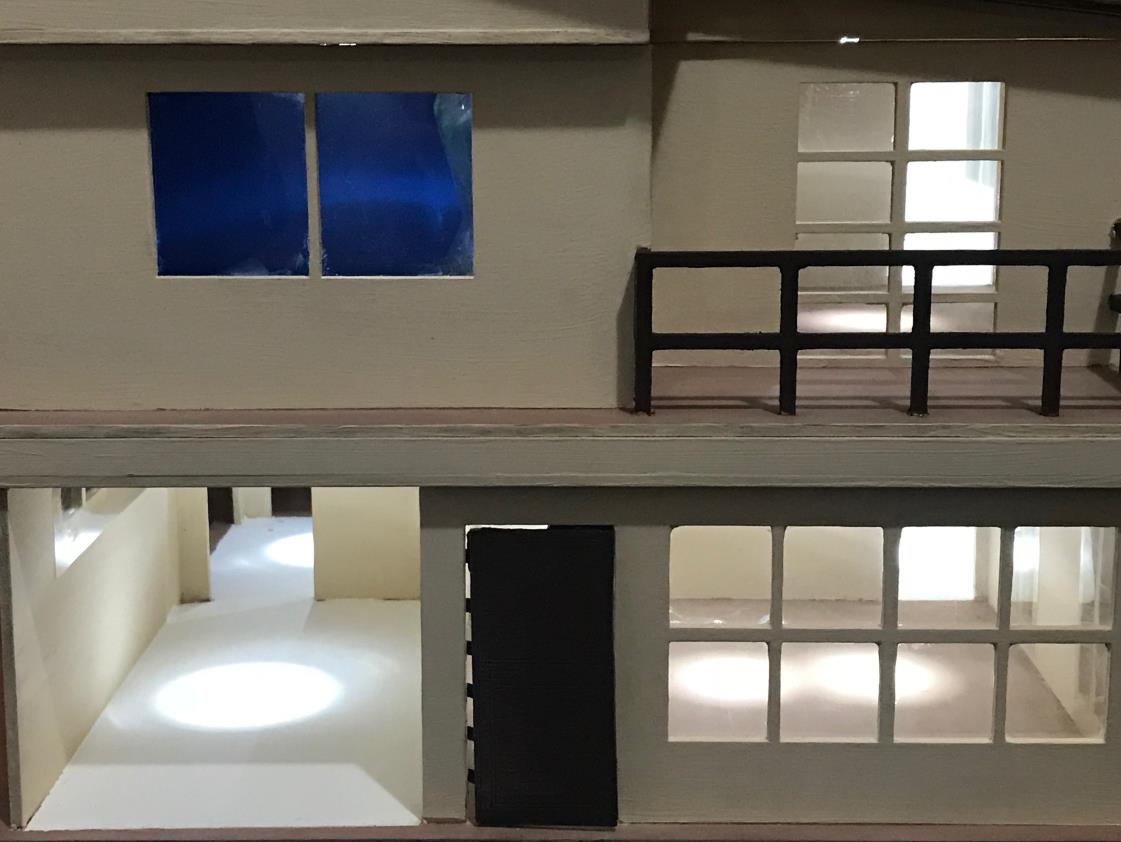
\includegraphics[scale=0.4]{Imagens/maquete_leandro_dallarosa.png}
    \legend{Fonte: \cite{ref:031}.}
    \label{fig:maquete_leandro_dallarosa}
\end{figure}

% -----------------------------------------------------------------------------
% Capítulo 2.6.2 - PROTÓTIPO DE AUTOMAÇÃO RESIDENCIAL UTILIZANDO UMA ASSISTENTE DE VOZ
% -----------------------------------------------------------------------------
\subsection{\textit{Creating an Alexa voice controlled IoT using a Raspberry Pi}}\label{subsection:creating_an_alexa_voice_controlled_iot_using_a_raspberry_pi}

Esse projeto foi desenvolvido em 2019 pelo YouTuber John Allwork com o objetivo de demonstrar um Raspberry Pi sendo controlado por voz através da Alexa \cite{ref:032}. O projeto conta com uma sequência de vídeos e documentação textual de como criar o seu nó IoT na rede AWS, carregar o código exemplo no AWS Lambda, criar habilidades na Alexa developer console e carregar o \textit{firmware} em um Raspberry Pi 4.

A \autoref{fig:testing_our_raspberrypi_thing} mostra uma captura de tela do vídeo 5 da sequência de vídeos do projeto do YouTuber John Allwork.

\begin{figure}[htbp]
    \centering
    \caption{Captura de tela do vídeo 5 da sequência de vídeos do projeto ``\textit{Creating an Alexa voice controlled IoT using a Raspberry Pi}''.}
    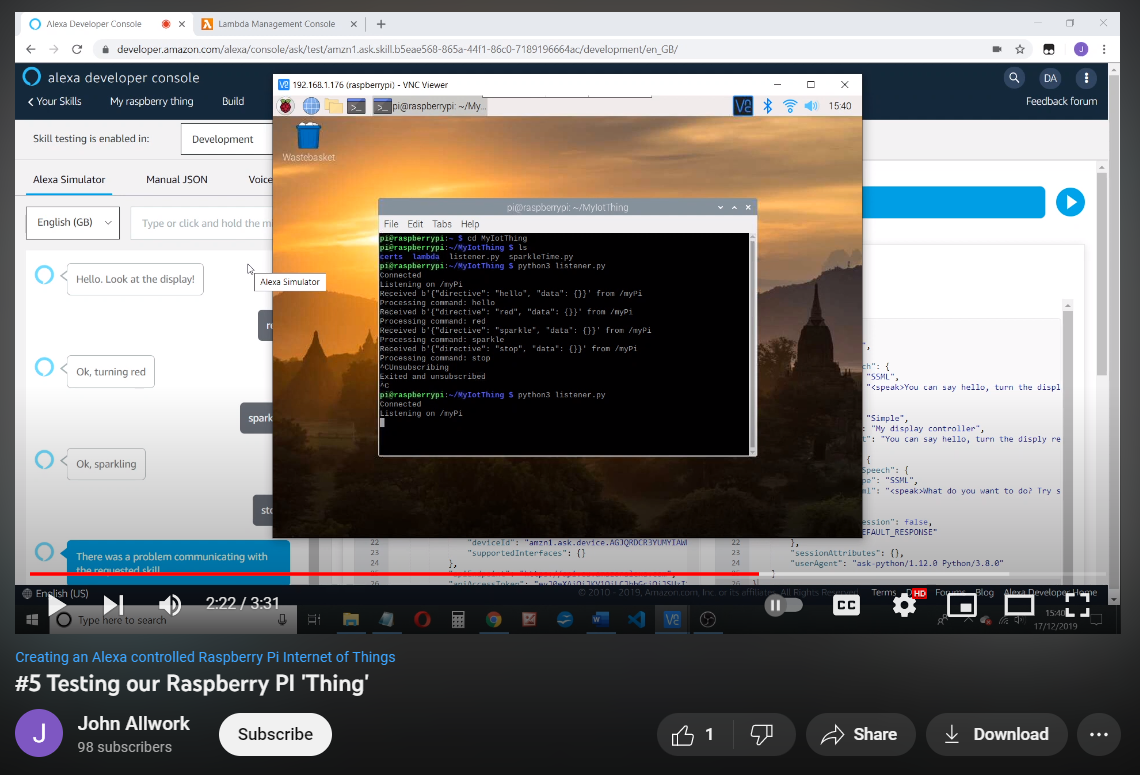
\includegraphics[scale=0.75]{Imagens/testing_our_raspberrypi_thing.png}
    \legend{Fonte: Produzido pelo autor (2022).}
    \label{fig:testing_our_raspberrypi_thing}
\end{figure}
